\chapter{Theoretical Background and Design Rationale}
\label{chap:ch2}

\tolerance=9999
\emergencystretch=3em

\par This chapter establishes the theoretical foundations on which the peer-assisted
streaming system rests, and justifies each major architectural decision in light of
those foundations.  The discussion proceeds from the broad landscape of content
delivery models, through the specifics of chunk-based media transport, peer
connectivity via WebRTC, and the prefix caching strategy, before arriving at a
formal bandwidth cost model that motivates the design as a whole.

% ─────────────────────────────────────────────────────────────────────────────
\section{Content Delivery Architecture Models}
\label{sec:delivery-models}

\par The way audio or video data travels from a content provider to a consumer has
evolved through several distinct architectural paradigms, each with a different
cost and latency profile.  Understanding these paradigms, and their respective
failure modes at scale, is a prerequisite for appreciating the design choices made
in this work.

\subsection{The Traditional Client-Server Model and its Cost Ceiling}
\label{subsec:client-server}

\par In the simplest delivery architecture, each client opens a direct TCP connection
to the origin server and streams data at the required bitrate.  The model is easy to
reason about: the server holds all content, all bandwidth is paid by the provider,
and clients are purely passive consumers.  The fundamental problem is that server
egress cost grows linearly with the number of concurrent listeners.  Formally, if a
song of size $S$ bytes is listened to by $N$ concurrent users, the total egress
volume is

\begin{equation}
  B_{\text{server}} = N \cdot S.
  \label{eq:server-cost}
\end{equation}

\par For large $N$, this is commercially unsustainable.  Cloud egress pricing from
major providers (AWS, GCP, Azure) is typically charged per gigabyte transferred out
of the data centre.  At a library of millions of tracks and tens of millions of daily
active users, equation~\eqref{eq:server-cost} translates directly into the
multi-hundred-million-dollar infrastructure bills observed at providers such as
Spotify \cite{spotify_google}.

\subsection{Content Delivery Networks}
\label{subsec:cdn}

\par Content Delivery Networks (CDNs) address the latency dimension of the
client-server problem by replicating popular content to geographically distributed
\emph{edge nodes}.  A client is routed to the nearest edge node, reducing the
round-trip time and often improving throughput.  However, CDNs do not reduce the
\emph{total} egress cost: every byte still originates from infrastructure owned or
leased by the provider and is billed at egress rates.  The replication itself
incurs additional intra-CDN transfer fees for warming edge caches.  Furthermore,
the replication model is poorly suited to long-tail content (rarely played tracks)
that must be stored at all edge locations despite being requested only occasionally.
CDNs therefore partially solve the latency problem while leaving the cost problem
intact.

\subsection{Peer-Assisted Hybrid Delivery}
\label{subsec:hybrid}

\par The peer-assisted model augments the client-server baseline with
device-to-device transfer.  After a client downloads a portion of content from the
server, it advertises that portion to other interested clients and serves it
directly over a P2P channel.  The server's role shifts from serving every byte to
serving only the initial fraction that bootstraps each new client into the swarm.
The theoretical minimum server egress for a swarm of $N$ users is achieved when
the first client downloads the full content from the server and every subsequent
client downloads entirely from peers:

\begin{equation}
  B_{\text{hybrid}}^{\min} = S + (N-1) \cdot \epsilon,
  \label{eq:hybrid-min}
\end{equation}

where $\epsilon$ is the per-client server overhead for bootstrapping (the prefix).
In practice, churn, clients leaving before peers can download from them, raises this
floor, but the gain over equation~\eqref{eq:server-cost} remains substantial even
under realistic churn rates.  Figure~\ref{fig:cost-comparison} illustrates the
asymptotic difference between the two models.

\begin{figure}[htbp]
\centering
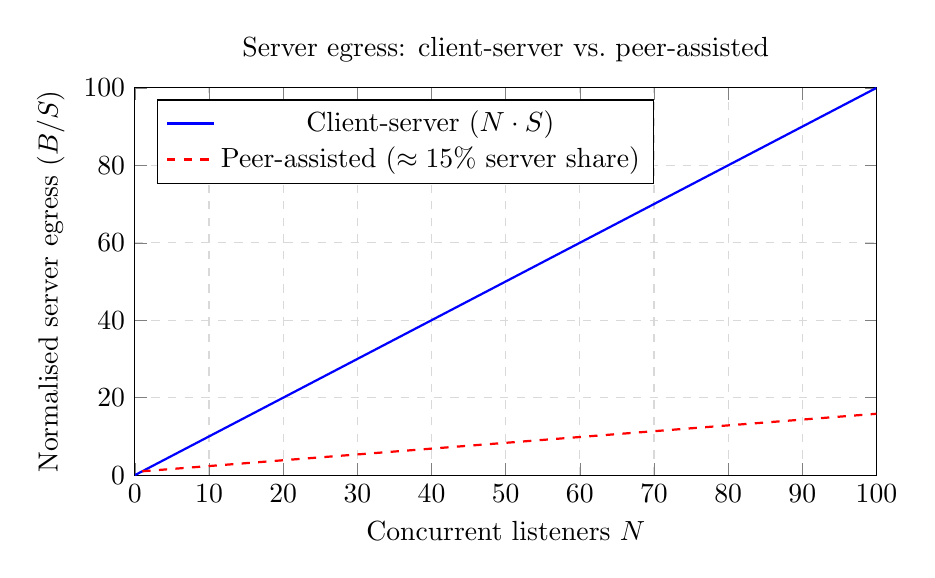
\begin{tikzpicture}
  \begin{axis}[
    width=11cm, height=6.5cm,
    xlabel={Concurrent listeners $N$},
    ylabel={Normalised server egress ($B / S$)},
    xmin=0, xmax=100,
    ymin=0, ymax=100,
    grid=both,
    grid style={dashed, gray!30},
    title={Server egress: client-server vs.\ peer-assisted},
    legend pos=north west,
  ]
    % Pure server: y = x
    \addplot[blue, thick, domain=0:100, samples=2]
      {x};
    \addlegendentry{Client-server ($N \cdot S$)}

    % Hybrid: y = 1 + (x-1)*0.15  (15% server fraction after bootstrap)
    \addplot[red, thick, dashed, domain=1:100, samples=100]
      {1 + (x-1)*0.15};
    \addlegendentry{Peer-assisted ($\approx 15\%$ server share)}
  \end{axis}
\end{tikzpicture}
\caption{Theoretical server egress volume as a function of concurrent listeners,
         contrasting pure client-server delivery with a peer-assisted model that
         routes 85\,\% of data through P2P channels.}
\label{fig:cost-comparison}
\end{figure}

\par The hybrid model introduces design constraints that the pure server model
avoids.  Peers must be discoverable, must hold relevant data at the right moment,
and must be reachable despite NAT and firewall boundaries.  The remainder of this
chapter addresses each of these constraints in turn.

% ─────────────────────────────────────────────────────────────────────────────
\section{Chunk-Based Streaming and Content-Addressed Storage}
\label{sec:chunk-theory}

\par The granularity at which content is partitioned has profound consequences for
both delivery efficiency and storage economy.  This section develops the theoretical
argument for fixed-size, content-addressed chunks as the primary storage and
transfer unit.

\subsection{Fixed-Size Partitioning}
\label{subsec:fixed-chunks}

\par Dividing an audio file into fixed-size blocks of $C$ bytes produces
$\lceil S / C \rceil$ chunks.  Fixed sizing, as opposed to variable-length
segmentation, has several practical advantages for a P2P system:

\begin{itemize}
  \item \textbf{Uniform scheduling}: a requester can ask any peer for ``chunk $i$''
        without needing to know the byte boundaries of that segment; the boundaries
        are implicit from $i \times C$.

  \item \textbf{Predictable buffer arithmetic}: the audio playback layer can
        translate byte-range requests into chunk indices with integer arithmetic,
        avoiding the need to transmit segment boundary tables.

  \item \textbf{Bounded memory}: a receiving buffer of fixed capacity (measured in
        chunks) is also bounded in bytes, enabling deterministic memory planning.
\end{itemize}

\par The choice of chunk size $C$ is a tuning parameter that trades latency for
overhead.  Smaller chunks reduce the time-to-first-byte of a P2P transfer but
increase the number of round trips and index entries.  Larger chunks amortise
per-request overhead but increase the granularity at which a peer can serve
partial data.  A size of $C = 65\,536$ bytes (64~KiB) sits at the intersection of
efficient I/O alignment (a power-of-two multiple of typical disk and network buffer
sizes) and practical P2P scheduling granularity.  At a typical audio bitrate of
320\,kbps for a high-quality MP3, one chunk holds approximately 1.6 seconds of
audio, giving a resolution that is finer than human perception of buffering
artefacts (${\sim}2{-}3$ seconds) while still being coarse enough to keep the
chunk count per song in the tens to low hundreds.

\subsection{Content-Addressed Storage and Deduplication}
\label{subsec:cas}

\par Content-addressed storage (CAS) is a paradigm in which the \emph{identity}
of a data block is derived from its \emph{content}, rather than from an externally
assigned identifier or file path.  The canonical mechanism is to use a
cryptographic hash of the block's bytes as its key.  This thesis uses SHA-256,
which maps any input to a 256-bit digest and has a collision probability of
approximately $2^{-256}$, negligible in any practical context.

\par The deduplication benefit of CAS is directly applicable to music libraries.
Many tracks share silence segments, common fade-outs, or identical album-art
headers embedded in audio containers.  With CAS, all such identical 64~KiB blocks
are stored once regardless of how many songs reference them.  More formally, if $k$
distinct byte-level 64~KiB blocks occur across all songs, the storage footprint is
$k \cdot C$ bytes, which is at most $\sum_i S_i$ (the sum of all song sizes) and
often substantially less.

\subsection{Hash-Based Integrity Verification}
\label{subsec:integrity}

\par The same SHA-256 digest that deduplicates storage also functions as an
integrity check.  Because the digest is precomputed at upload time and stored in
the chunk manifest, a client receiving chunk $i$ from \emph{any} source, origin
server or peer, can recompute the SHA-256 of the received bytes and compare it to
the expected value.  A mismatch unambiguously indicates corruption or deliberate
tampering.  This property is critical in the peer-assisted model, where a
misbehaving or compromised peer could otherwise inject corrupted audio data.  The
verification cost is negligible relative to network latency: a 64~KiB SHA-256
computation completes in under a microsecond on modern hardware \cite{sha256_perf}.

% ─────────────────────────────────────────────────────────────────────────────
\section{WebRTC as a Peer-to-Peer Transport Layer}
\label{sec:webrtc-theory}

\par Web Real-Time Communication (WebRTC) is an open standard that enables
browser and native applications to establish direct peer-to-peer connections
for audio, video, and arbitrary binary data, without requiring a dedicated relay
server for the media itself \cite{webrtc_spec}.  Its adoption in this system is
motivated by three properties: ubiquity (native support in all major browsers and
Flutter via the \texttt{flutter\_webrtc} package), NAT traversal capability, and
support for ordered reliable data channels.

\subsection{NAT Traversal: ICE, STUN, and TURN}
\label{subsec:nat-traversal}

\par The majority of end-user devices sit behind Network Address Translation (NAT)
gateways, which rewrite the source IP address and port of outgoing packets.  A
device behind NAT cannot be contacted directly by an external peer using its
private address; a traversal mechanism is required.

\par Interactive Connectivity Establishment (ICE) \cite{rfc8445} is the WebRTC
framework for discovering and negotiating a viable network path between two peers.
ICE collects \emph{candidates}, possible transport addresses, from three sources:

\begin{enumerate}
  \item \textbf{Host candidates}: the device's own network interface addresses.
  \item \textbf{Server-reflexive candidates}: the public IP/port mapping created
        by the NAT, discovered by querying a STUN (Session Traversal Utilities
        for NAT \cite{rfc8489}) server.
  \item \textbf{Relayed candidates}: addresses on a TURN (Traversal Using Relays
        around NAT \cite{rfc8656}) relay server, used only when direct
        connectivity fails.
\end{enumerate}

\par In most residential NAT configurations, a STUN exchange suffices: both peers
learn their server-reflexive addresses and use UDP hole-punching to establish a
direct path.  TURN relaying is reserved for symmetric NATs and enterprise
firewalls; its cost is significantly higher but its traffic volume is bounded
because the system falls back to server delivery rather than TURN when P2P fails.
Figure~\ref{fig:ice-flow} illustrates the ICE candidate exchange sequence.

\begin{figure}[htbp]
\centering
\resizebox{\textwidth}{!}{%
\begin{tikzpicture}[
  node distance=1.3cm and 3.5cm,
  box/.style={rectangle, draw, rounded corners=3pt,
              minimum width=2.4cm, minimum height=0.8cm,
              font=\small, align=center},
  srv/.style={box, fill=orange!15},
  peer/.style={box, fill=blue!10},
  stun/.style={box, fill=green!10},
  arr/.style={-{Stealth}, thick},
  darr/.style={-{Stealth}, thick, dashed}
]
  \node[peer]  (pA)   {Peer A};
  \node[stun, right=of pA]  (stun) {STUN\\Server};
  \node[srv,  right=of stun] (sig)  {Signaling\\Server};
  \node[peer, right=of sig]  (pB)   {Peer B};

  % STUN exchange
  \draw[arr]  (pA) -- node[above, font=\scriptsize]{Binding Req.} (stun);
  \draw[arr]  (stun.west) to[bend left=20]
              node[below, font=\scriptsize]{Reflexive addr.} (pA.south);

  % Candidate exchange via signaling
  \draw[darr] (pA.north) to[bend left=12]
              node[above, font=\scriptsize]{OFFER + candidates} (sig.north west);
  \draw[darr] (sig.north east) to[bend left=12]
              node[above, font=\scriptsize]{OFFER + candidates} (pB.north);
  \draw[darr] (pB.south) to[bend left=12]
              node[below, font=\scriptsize]{ANSWER + candidates} (sig.south east);
  \draw[darr] (sig.south west) to[bend left=12]
              node[below, font=\scriptsize]{ANSWER + candidates} (pA.south);

  % Direct P2P after ICE
  \draw[arr, red, very thick] (pA.east) to[bend right=35]
              node[below, font=\scriptsize, red]{\textbf{Direct P2P}} (pB.west);
\end{tikzpicture}%
}
\caption{ICE candidate exchange using a STUN server and signaling relay,
         resulting in a direct peer-to-peer data path.}
\label{fig:ice-flow}
\end{figure}

\subsection{Data Channels for Binary Chunk Transfer}
\label{subsec:data-channels}

\par WebRTC Data Channels provide an SCTP-over-DTLS transport that supports both
reliable ordered delivery (analogous to TCP) and unreliable unordered delivery
(analogous to UDP).  For audio chunk transfer, reliable ordered delivery is the
appropriate choice: audio data must arrive without corruption and the chunk
boundary semantics depend on receiving complete 64~KiB blocks.  Unlike TCP,
however, SCTP's head-of-line blocking is confined to a single stream, so a stalled
chunk request on one data channel does not block data channels to other peers.

\par The binary message format over a data channel is deliberately minimal.  A
fixed 8-byte header encodes the song identifier (4 bytes, big-endian) and the
chunk index (4 bytes, big-endian), followed directly by the audio payload.  The
choice of a fixed-length header over a framing protocol such as Protocol Buffers
is motivated by the fact that chunk transfers are entirely homogeneous, no
multiplexing of different message types is needed on a single data channel, so a
length-prefixed header would add overhead without benefit.

\subsection{Signaling and the Role of the Server}
\label{subsec:signaling-role}

\par WebRTC requires an \emph{out-of-band signaling channel} for the exchange of
SDP (Session Description Protocol) offer/answer payloads and ICE candidates.
This channel is the \emph{only} persistent server dependency in the P2P path; once
the data channel is open, the server is no longer involved in media transfer.  The
choice of WebSocket as the signaling transport aligns well with the existing server
infrastructure and allows the same connection to carry library synchronisation
events and peer discovery messages, reducing the number of persistent connections
each client must maintain.

% ─────────────────────────────────────────────────────────────────────────────
\section{The Prefix Caching Strategy}
\label{sec:prefix-theory}

\par A naive peer-assisted streaming system faces an irresolvable bootstrapping
problem: a new client cannot receive data from peers until it has connected to
them, and connecting to peers requires the ICE negotiation described in
Section~\ref{sec:webrtc-theory}, which takes hundreds of milliseconds.  During
this window, the audio player has no data to decode and playback cannot start.

\subsection{Playback Latency Decomposition}
\label{subsec:latency-decomp}

\par The total startup latency $T_{\text{start}}$ for a client requesting a song
can be decomposed as:

\begin{equation}
  T_{\text{start}} = T_{\text{resolve}} + T_{\text{buffer}},
  \label{eq:latency}
\end{equation}

where $T_{\text{resolve}}$ is the time to acquire enough data for the audio decoder
to begin, and $T_{\text{buffer}}$ is the time to buffer a sufficient lookahead to
avoid starvation during subsequent streaming.  In the P2P model, $T_{\text{resolve}}$
is dominated by the WebRTC connection setup time ($T_{\text{ICE}} \approx
200{-}500$\,ms) plus the first chunk transfer latency.  An unmitigated peer-first
strategy would therefore introduce a mandatory 200–500 ms delay even for popular
songs with many available peers.

\par The prefix strategy eliminates this delay by decoupling the initial buffer fill
from peer discovery.  The client simultaneously (a) fetches a fixed prefix of the
song from the origin server over HTTP and (b) initiates peer discovery via the
signaling server.  Playback begins as soon as the prefix arrives; by the time the
prefix is consumed, peer connections are typically established and the remainder
of the song is served from peers.

\subsection{Choosing the Prefix Threshold}
\label{subsec:prefix-threshold}

\par The prefix must be large enough that $T_{\text{buffer}}$ covers the full peer
negotiation time $T_{\text{ICE}}$ plus the first peer response time.  Let $r$ be
the audio bitrate in bytes per second and $P$ be the prefix size in bytes.  The
prefix sustains playback for $P / r$ seconds.  For this to cover ICE negotiation
and an initial P2P timeout of $T_{\text{p2p}}$ seconds, we require:

\begin{equation}
  \frac{P}{r} > T_{\text{ICE}} + T_{\text{p2p}}.
  \label{eq:prefix-condition}
\end{equation}

\par At $r = 40\,960$ bytes/s (320\,kbps), $T_{\text{ICE}} = 500$\,ms, and
$T_{\text{p2p}} = 1000$\,ms, equation~\eqref{eq:prefix-condition} gives
$P > 61\,440$ bytes, less than one chunk.  The chosen prefix of eight chunks
(524\,288 bytes, sustaining $\approx 12.8$\,s of playback) provides a generous
safety margin that accommodates slow NAT environments, CDN cold-starts on the
server prefix fetch, and the 16-chunk lookahead prefetch window.  The same eight
chunks are used as the boundary below which the client unconditionally fetches
from the server, aligning the prefix delivery endpoint with the P2P onset point
and making the server's prefix endpoint a natural cache target.

\subsection{Proactive Queue Prefetching}
\label{subsec:proactive-theory}

\par A user listening to a playlist will transition between songs with negligible
delay only if the next song's startup sequence (prefix fetch and peer negotiation)
completes before the current song ends.  Proactive prefetching addresses this by
initiating prefix downloads for the next $k$ songs in the queue while the current
song is playing.  The bandwidth overhead is bounded: the total proactive download
is $k \cdot P$ bytes, which for $k = 5$ and $P = 524\,288$ bytes totals
approximately 2.5~MiB, a modest background cost compared to the elimination of any
inter-song latency.

% ─────────────────────────────────────────────────────────────────────────────
\section{Bandwidth Cost Model}
\label{sec:cost-model}

\par Having established the individual mechanisms, this section synthesises them
into a formal cost model that quantifies the expected reduction in server egress
and motivates the specific parameter choices made in the implementation.

\subsection{Theoretical Offload Ratio}
\label{subsec:offload-ratio}

\par Define the \emph{offload ratio} $\rho$ as the fraction of total bytes served
by peers rather than the origin server.  For a swarm of $N$ simultaneous listeners
of a song of size $S$, each listener requires one prefix of size $P$ from the
server.  Assuming all non-prefix bytes are served by peers (the ideal case), the
server egress is $N \cdot P$ and the total bytes consumed is $N \cdot S$:

\begin{equation}
  \rho = 1 - \frac{P}{S} = 1 - \frac{8C}{S},
  \label{eq:offload-ratio}
\end{equation}

where $C = 65\,536$ bytes.  For a 4-minute song at 320\,kbps, $S \approx 9.6$\,MB
and $8C \approx 0.52$\,MB, giving $\rho \approx 94.6\,\%$.  Even a 1-minute track
($S \approx 2.4$\,MB) yields $\rho \approx 78.3\,\%$.  These figures represent
upper bounds; in practice, churn and cold starts reduce the achievable ratio, but
the asymptotic behaviour in equation~\eqref{eq:server-cost} is converted from
$O(N)$ to $O(1)$ in server egress per unit time, the cost becomes independent of
swarm size.

\subsection{Design Trade-offs and Parameter Sensitivity}
\label{subsec:tradeoffs}

\par The model reveals several trade-offs that informed the implementation:

\begin{itemize}
  \item \textbf{Prefix size vs.\ offload ratio}: A larger prefix reduces $\rho$
        (more server cost) but increases startup robustness.  The chosen eight
        chunks balance these concerns, as shown by equation~\eqref{eq:prefix-condition}.

  \item \textbf{P2P timeout vs.\ stall probability}: A longer timeout gives slow
        peers more time to respond, increasing the offload ratio, but risks
        audible stalls if the audio player exhausts its lookahead buffer.  The
        one-second timeout, combined with a 16-chunk ($\approx 1$\,MB) lookahead,
        ensures the buffer survives one failed peer request before the server
        fallback path returns data.

  \item \textbf{Chunk size vs.\ overhead}: Halving $C$ to 32~KiB would double
        the chunk count and index size while reducing the per-chunk transfer
        latency.  Doubling $C$ to 128~KiB would reduce overhead but coarsen
        the P2P scheduling granularity, making it harder for a peer to serve
        partial data if it has only downloaded part of a large block.  The
        64~KiB value sits at a practical optimum for the target content
        (320\,kbps MP3 and FLAC).

  \item \textbf{Swarm size and peer density}: The model assumes at least one
        peer with a given chunk is reachable within the P2P timeout.  For
        long-tail songs with very few listeners, peers may be absent and the
        system degrades gracefully to pure server delivery.  No additional
        logic or user experience penalty is incurred in this case: the
        server fallback is always available and the one-second timeout is
        the only overhead.
\end{itemize}

\par Table~\ref{tab:param-summary} summarises the key parameters and their
theoretical justification.

\begin{table}[htbp]
\centering
\begin{tabular}{|p{3.8cm}|p{2.2cm}|p{7.5cm}|}
\hline
\textbf{Parameter} & \textbf{Value} & \textbf{Justification} \\
\hline
Chunk size $C$ & 65\,536 B & Power-of-two I/O alignment; $\approx 1.6$\,s of 320\,kbps audio \\
\hline
Prefix chunks & 8 & Covers $T_{\text{ICE}} + T_{\text{p2p}}$ at max audio bitrate with safety margin \\
\hline
P2P timeout & 1\,000\,ms & Balances peer-wait cost against 16-chunk buffer capacity \\
\hline
Lookahead & 16 chunks & $\approx 1$\,MiB; absorbs one full P2P timeout without stall \\
\hline
RAM cache size & 15 chunks & Absorbs overlapping range requests from audio player \\
\hline
Proactive prefetch & 5 songs & Eliminates inter-song latency; adds $\approx 2.5$\,MiB background load \\
\hline
State save interval & 30\,s & Limits server write load while bounding session data loss \\
\hline
\end{tabular}
\caption{Key system parameters and their theoretical justification.}
\label{tab:param-summary}
\end{table}
